\documentclass[text01.tex]{subfiles}
\begin{document}
%
% section 1.7
%
\section{\ruby{質問}{しつもん}フォーム}

わからないことや、\ruby{質問}{しつもん}したいことがあれば、そのままにしておかないで、\ruby{積極的}{せっきょくてき}に
\ruby{質問}{しつもん}しましょう！
\ruby{質問}{しつもん}フォームを使うと、\ruby{授業}{じゅぎょう}でわからなかったことや、\ruby{確認}{かくにん}したいことなどを、
お家からでも、ホームページを通して\ruby{質問}{しつもん}できます。
たくさん\ruby{質問}{しつもん}して、わからないことを\ruby{解決}{かいけつ}しましょう。
\bigskip

{\bf \ruby{質問}{しつもん}フォームの使い方}

\noindent%
  \begin{minipage}[t]{0.44\columnwidth}
    \textcircled{\scriptsize{1}}\\
    ブラウザで、「\ruby{授業}{じゅぎょう}で使うホームページリスト」（\texttt{links.html}）を開きましょう。
    \ul{子どもIT未来塾質問フォーム}をクリックしてください。
    （スマートフォン等からは、\texttt{https://bit.ly/2NHiVgi}でアクセスできます。）
  \end{minipage}\hfill
  %
  \begin{minipage}[t]{0.55\columnwidth}
    \centering
    \vbox to 0pt{\vskip-3mm
      % 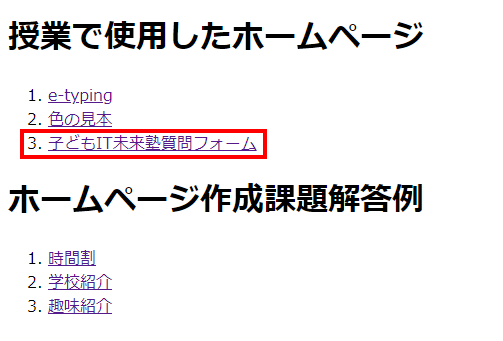
\includegraphics[keepaspectratio, height=55mm]{../../asset/image/textbook-img245.png}
      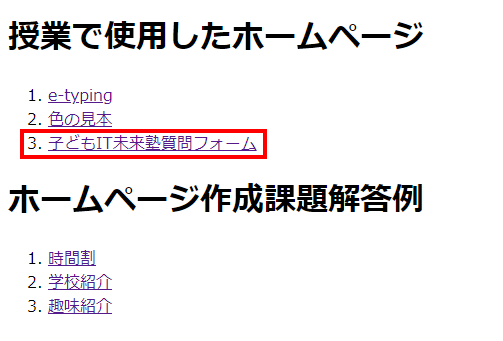
\includegraphics[keepaspectratio, width=0.8\linewidth]{../../asset/image/textbook-img245.png}
    \vss}
    \vspace{50mm}
  \end{minipage}
%
\begin{minipage}[t]{0.44\columnwidth}
  \textcircled{\scriptsize{2}}\\
  \ruby{質問}{しつもん}フォームが\ruby{表示}{ひょうじ}されます。
  メールアドレス、名前、グループの先生の名前、ぎもんに思っていることを入力します。
  必要に応じて、ぎもんに思っている場所の画像も追加できます。
  入力が終わったら、最後に質問ボタンをクリックします。
\end{minipage}\hfill
%
\begin{minipage}[t]{0.55\columnwidth}
  \centering
  \vbox to 0pt{\vskip-3mm
    % 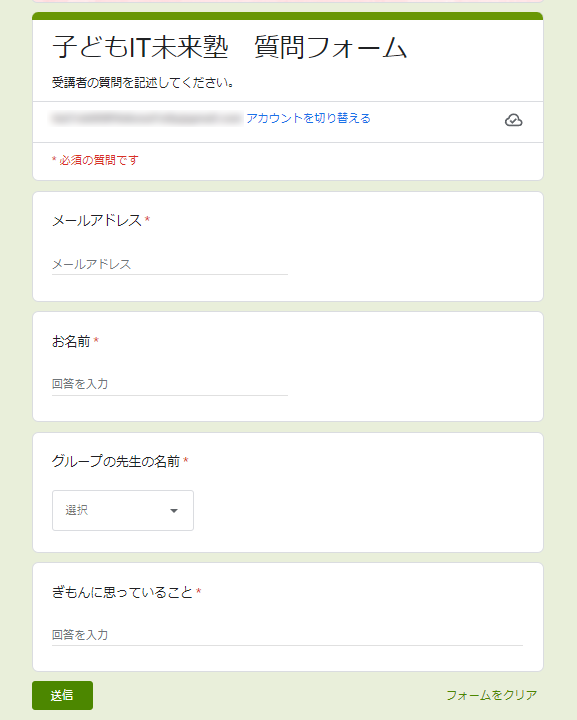
\includegraphics[keepaspectratio, height=80mm]{../../asset/image/textbook-img246.png}
    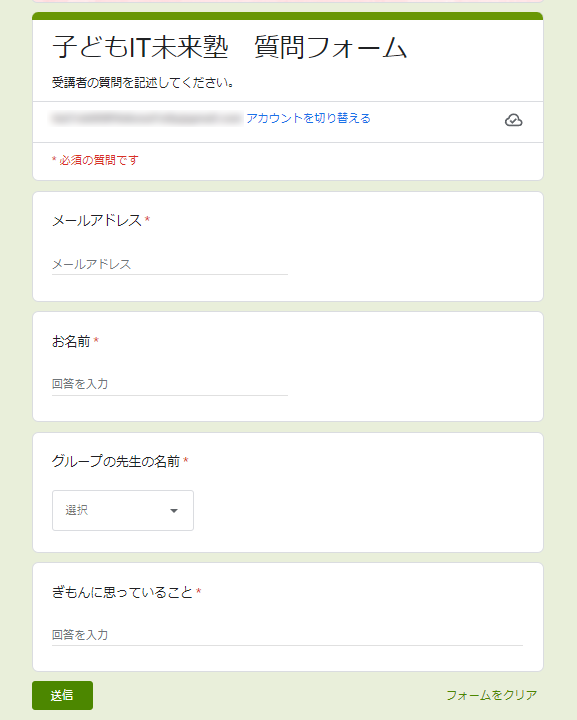
\includegraphics[keepaspectratio, width=0.8\linewidth]{../../asset/image/textbook-img246.png}
  \vss}
  \vspace{95mm}
\end{minipage}
%
\begin{minipage}[t]{0.44\columnwidth}
  \textcircled{\scriptsize{3}}\\
  右の画面が表示されたら、質問は完了です。
  メールアドレスのらんに入力したアドレスに、グループの先生から回答メールがきます。
  回答には、数日かかる場合もあります。
\end{minipage}\hfill
%
\begin{minipage}[t]{0.55\columnwidth}
  \centering
  \vbox to 0pt{\vskip-3mm
    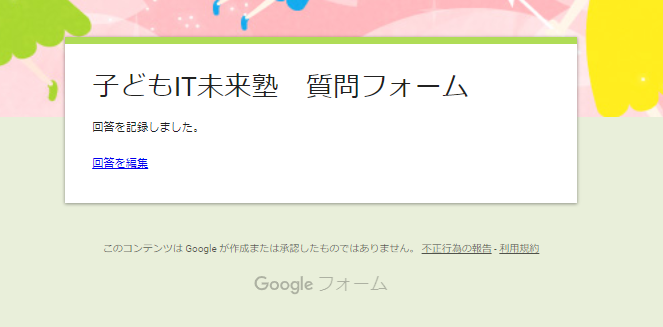
\includegraphics[keepaspectratio, width=0.8\linewidth]{../../asset/image/textbook-img247.png}
  \vss}
  \vspace{40mm}
\end{minipage}
%



% \centering
% \begin{figure}[H]
%   \begin{minipage}{\textwidth}
%     {\upshape
%       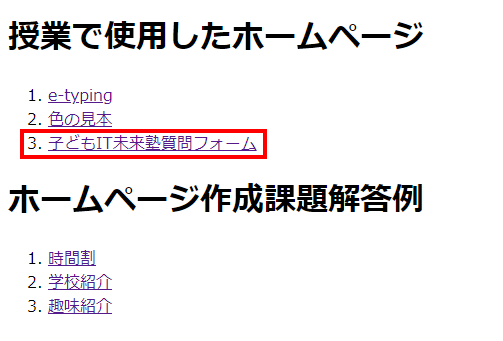
\includegraphics[width=0.9\textwidth]{../../asset/image/textbook-img245.png}
%       \caption{ホームページリストより\ruby{質問}{しつもん}フォームを開く}\label{fig:51}
%     }
%   \end{minipage}  
% \end{figure}


% \bigskip

% \bigskip
% \clearpage
% 2.
% \ruby{質問}{しつもん}フォーム(図~\ref{fig:52})が\ruby{表示}{ひょうじ}されます

% \centering
% \begin{figure}[H]
%   \begin{minipage}{\textwidth}
%     {\upshape
%       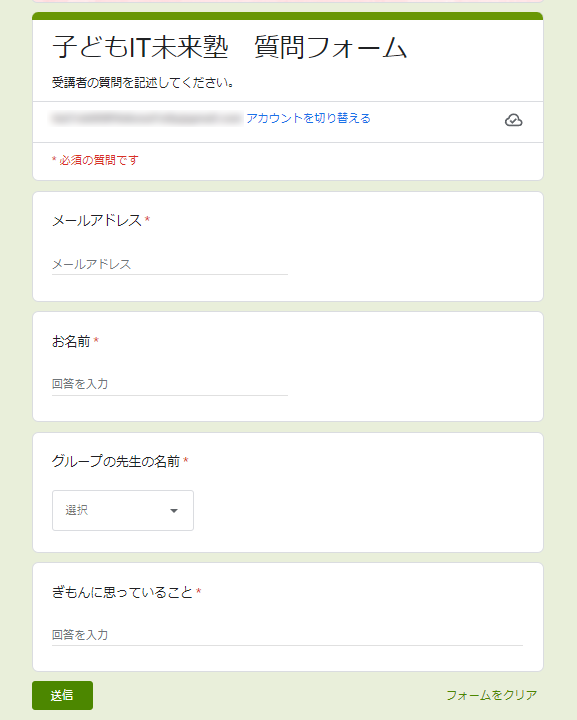
\includegraphics[width=0.7\textwidth]{../../asset/image/textbook-img246.png}
%       \caption{\ruby{質問}{しつもん}フォーム}\label{fig:52}
%     }
%   \end{minipage}  
% \end{figure}

% \flushleft

% \bigskip

% メールアドレス、お名前、グループの先生の名前、ぎもんに思っていることを入力します。
% 必要に\ruby{応}{おう}じて、ぎもんに思っている場所の\ruby{画像}{がぞう}を追加してください。

% {\bfseries
% 送信\textmd{を\ruby{押}{お}すと\ruby{質問}{しつもん}ができます。図~\ref{fig:53}の画面が出たら\ruby{質問}{しつもん}は\ruby{完了}{かんりょう}です。}}



% \centering
% \begin{figure}[H]
%   \begin{minipage}{\textwidth}
%     {\upshape
%       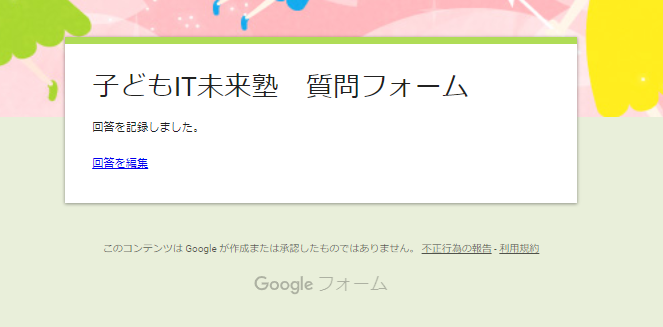
\includegraphics[width=0.45\textwidth]{../../asset/image/textbook-img247.png}
%       \caption{\ruby{質問}{しつもん}送信画面}\label{fig:53}
%     }
%   \end{minipage}  
% \end{figure}

% \flushleft
% メールアドレスのらんに入力したアドレスへグループの先生から回答メールがきます。
% メールが来るまで、しばらくお待ちください。数日かかる場合があります。

\end{document}
